\chapter{Fracture mechanic of wood}
\label{Chapter1}

\section{Introduction}

In this section, the mechanical properties of wood are reminded as well as the basics of fracture mechanics. 
Wood is a heterogeneous material and sensitive to moisture. Indeed, the humidity of wood is an important characteristic that has consequences for its physical and mechanical properties. The variation of the humidity will lead to variations of dimensions, shape, volume, density and thus of resistance of wood. 
The first theoretical developments of fracture mechanics were undertaken around 1940. Since then, the development of fracture mechanics has extended to materially and geometrically nonlinear problems, mixed-mode crack bifurcation problems, and more recently to composites, numerical solution techniques, and the state of the art in the design of various complex structures. The objective of applied fracture mechanics is to characterize the cracking behavior of structures using quantifiable parameters in the engineering sense, including stress, crack length, and material resistance to cracking.

This paper is based on the study of a softwood species that has a less complex structure than hardwoods. In this part, the material wood will be presented with its physical aspects and mechanical properties. Macroscopic and microscopic aspects will be reminded.
In addition, a look is taken at the mechanics of fracture with applications to the wood material. Essential notions will be recalled in order to understand the mechanics of linear fracture. We will see the different types of specimens used for similar studies, then the orthotropic mechanical fields. The last part of the chapter is devoted to the explanation of the DIC method.

\section{The wood material}

\subsection{Generalities about wood}

\subsubsection{The wood}

Wood is defined as 'a set of very resistant tissues that constitute the trunk, branches and roots of woody plants, formed by vessels conducting raw sap, fibres and parenchyma' (\ref{fig:fig1}). 


\begin{figure}[htp]
	\centering
	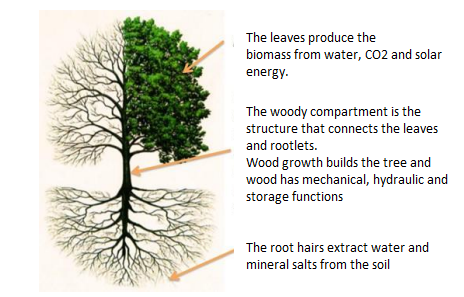
\includegraphics[width=8cm]{fig1}
	\caption{The main functions of the tree's wood, \cite{B.Thibaut}}
	\label{fig:fig1}
\end{figure}

The wood ensures in trees 3 main functions: the conduction of the raw sap from the roots to the branches, the mechanical support of the whole tree against its own weight and external forces, and the storage of nutrients such as starch. It is one of the few $100 \%$ natural materials. Its main chemical components are carbon, oxygen and hydrogen. Its use allows the limitation of greenhouse gas emissions and thus to fight against global warming. The tree absorbs carbon with which it manufactures the cells of the wood and rejects oxygen in the atmosphere. It is a natural material, renewable, transformable at low energy costs, recyclable, and biologically degradable. For construction, it has advantages and disadvantages presented in table \ref{fig:fig2}:

\begin{comment}
\begin{table} \centering
	\begin{tabular}{cc}
		\toprule % horizontal line at the top of the table
		 The advantages and disadvantages of wood  \\\midrule
		The advantages & The disavantages \\\midrule
		Solidity and lightness: the strength-to-weight ratio is high. Its low density (500kg/m3) allows the use of less massive foundations.& Natural material and therefore has a high variability \\\midrule  
		Good thermal insulation: it is much less conductive than steel or concrete and reduces thermal bridges in buildings. & Orthotropic material \\\midrule
		Renewable and aesthetic. & Moisture-sensitive material \\\midrule
		Chemically inert. & Material sensitive to attack by insects and fungi \\\midrule
		Good fire behaviour: there is no toxic release, little heat transmission to neighbouring parts. Wood has a higher load-bearing capacity than steel. & Material that requires regular maintenance. \\ 
		\bottomrule % horizontal line at the bottom of the table
	\end{tabular}
	\caption{Orders of magnitude of axial compressive strengths and elastic moduli}
	\label{fig:fig13}
\end{table}
\end{comment}

\begin{table}[htp]
	\centering
	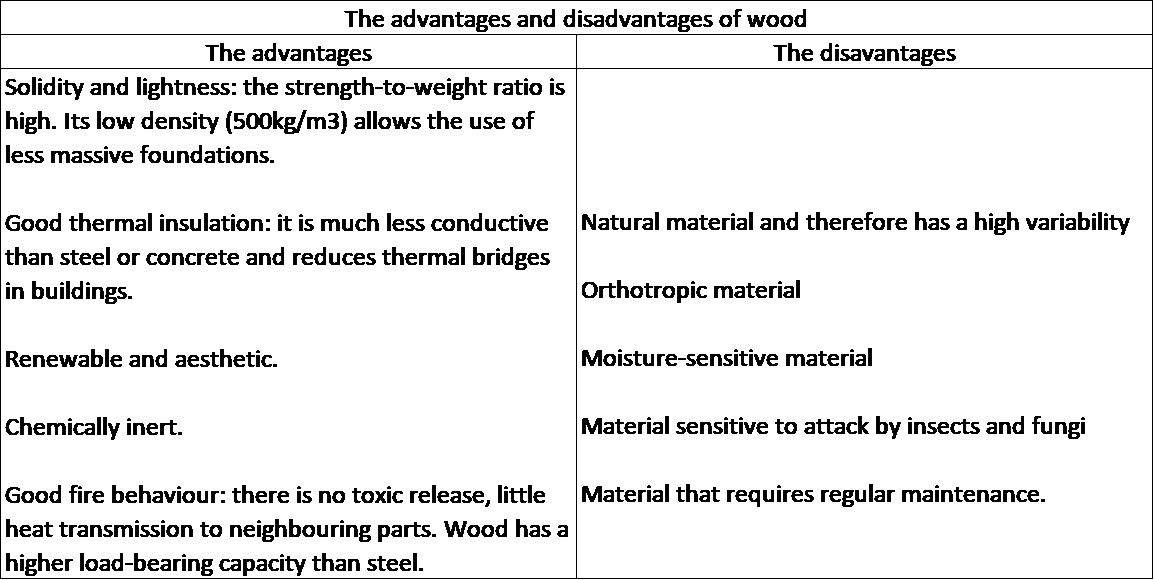
\includegraphics[width=12cm]{fig2}
	\caption{The advantages and disadvantages of wood}
	\label{fig:fig2}
\end{table}

\subsubsection{Two characteristics of the tree's wood}

Wood has two important characteristics: anisotropy and heterogeneity. Anisotropy is a direct consequence of heterogeneity.

\begin{itemize}
	\item It is heterogeneous in that it is composed of cells of different types and shapes. 
	\item It is anisotropic because its elements are oriented in several directions. Its mechanical and physical properties are not the same in all planes. The material is also orthotropic which means it has 3 preferred directions: longitudinal, radial and tangential.
\end{itemize}

In order to facilitate the studies on the physical and mechanical behaviours, we take as reference three types of sections as shown in figure \ref{fig:fig3} and defined them as follows:

\begin{itemize}
	\item Cross-section (T), perpendicular to the shaft of the tree (trunk). When we look at a freshly felled tree, we can easily imagine a cross-section with the annual growth rings at the end, which correspond to the woody material produced by the tree in spring or summer.
	\item Tangential section (L), longitudinal, in the direction of the wood grain, and perpendicular to the medullary rays centered on the core of the log. During the cutting of the log into logs (current cutting), the patterns of the faces of the first boards obtained are characteristic.
	\item Radial section (R), again longitudinal, and in the direction of the wood grain, but parallel
	to the rays. This section can be seen on trays cut near the heart.
\end{itemize}


\begin{figure}[htp]
	\centering
	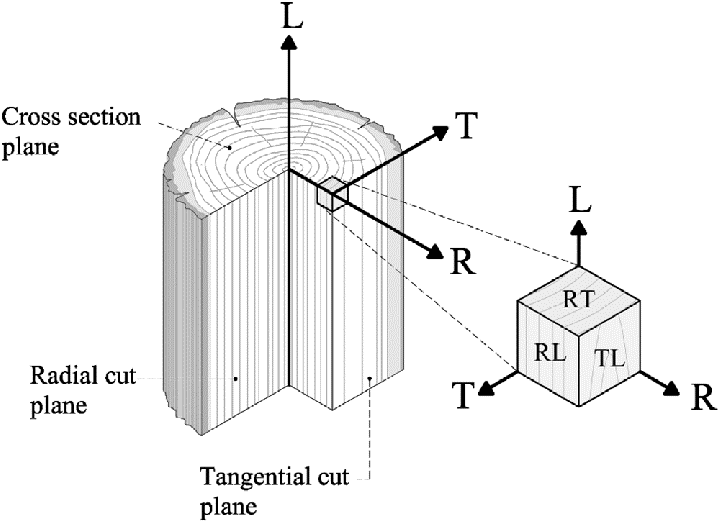
\includegraphics[width=10cm]{fig3}
	\caption{Main orthotropic directions and planes in Wood}
	\label{fig:fig3}
\end{figure}

\newpage

\subsection{Macroscopic and microscopic structure of wood}

\subsubsection{Macroscopic Scale}

The wood grows in concentric layers to the outside. It is this growth that creates heterogeneity; \cite{Seddik2006phd}. Figure \ref{fig:fig4} shows the different elements that participate in the growth of a tree:


\begin{figure}[htp]
	\centering
	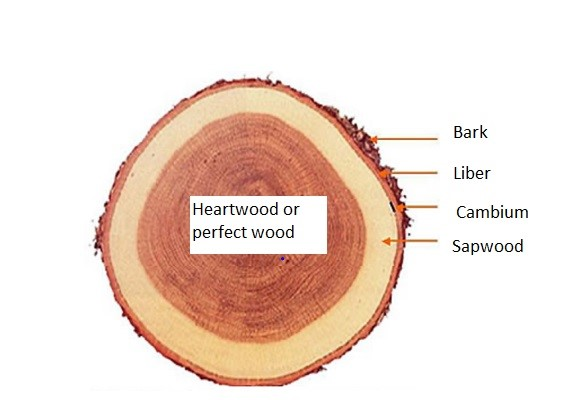
\includegraphics[width=10cm]{fig4}
	\caption{Sectional view of the wood}
	\label{fig:fig4}
\end{figure}

\begin{itemize}
	\item Outer bark: consists of dead cells and serves to protect the tree. It surrounds the tree to protect the cambium and the deep layer from climatic, animal or physical attack. 
	\item Inner bark (Liber): A layer of cells in which the elaborated (descending) sap circulates
	\item Cambium: Produces the bast towards the outside and the wood (xylem) towards the inside (growth tissue). This part can develop into sapwood or the next layer, the bark. It is therefore a particular part that explains the growth of the tree's circumference.
	\item Sapwood: Incompletely completed wood in which the raw sap circulates. The sap allows water and nutrients to be transmitted from the soil to all parts of the tree.
	\item Heartwood or perfect wood (dead cells) is the wood with the best mechanical properties. It is considered to be the dead part of the wood which is darker in colour than the other parts. It is the most used part of the tree for construction.
	\item Pith (heart) central part consisting of spongy tissue
\end{itemize}

There is sometimes a difference in colour between sapwood and heartwood (in the case of differentiated woods: oak, chestnut, pine, Douglas fir, larch). Sapwood is not or only slightly resistant to damage, whereas heartwood, which is not very impregnable, is naturally resistant. Conversely, for non-differentiated woods (fir, spruce, poplar, maple), the two parts are not visually distinguishable. However, there are different porosities and therefore different absorption capacities.

\subsubsection{Microscopic Scale}

Microscopically, there are two types of wood made up of different types of plant tissue: softwoods and hardwoods. Figure \ref{fig:fig5} presents microscopically these two categories of wood.

Softwoods are older than hardwoods and therefore have a simpler structure. They are made up of two main groups of cells: tracheids and parenchyma cells. The observation of these two types of cells shows the following configuration:

\begin{itemize}
	\item Tracheid fibers, having both support and conduction roles
	\item Rays: tracheid fibers and horizontal parenchyma
	\item Vertical parenchyma which ensure the distribution and storage of substances.
\end{itemize}

Hardwoods have more cell diversity than softwoods. They are composed of different cells: vessels, tracheids and parenchyma. The functions of support and conduction are performed by different cells:

\begin{itemize}
	\item Fibers (librifomes and tracheids): they are bundles of resistant cells, arranged in the axial direction, they ensure the rigidity and the mechanical resistance of wood. It is a bio composite made of cellulose, hemicellulose and ;
	\item Vessels: these are hollow cells that serve to conduct the raw sap from the roots to the leaves;
	\item Vertical parenchyma: this consists of parenchymal cells that contribute to the transport of nutrients. These parenchyma, associated with the vessels, give particular patterns to each species on the cross section;
	\item Woody rays (or medullary rays): these are horizontal parenchyma made up of thickened and lignified reserve cells with thickened and lignified walls. They accompany the vascular tissue. These cells participate in the support function of the tree. Their orientation is transverse and radiating from the longitudinal axis of the shaft.
\end{itemize}


\begin{figure}[htp]
	\centering
	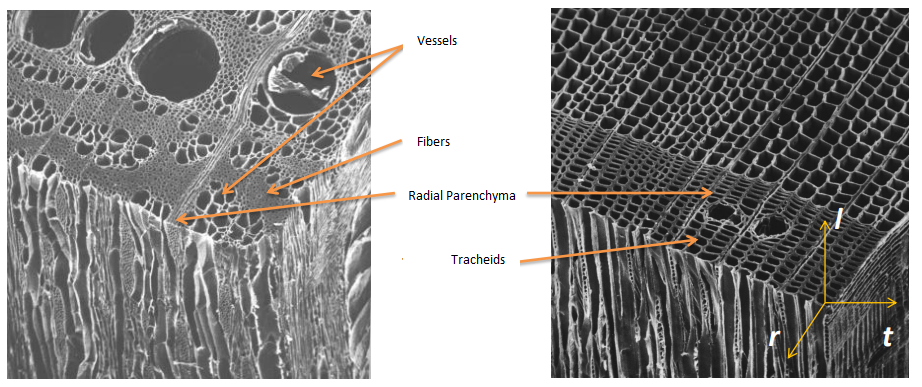
\includegraphics[width=12cm]{fig5}
	\caption{Microscopic section of hardwood and softwood, \cite{B.Thibaut}}
	\label{fig:fig5}
\end{figure}

\subsubsection{Chemical composition of wood}

Wood is a set of tissues of more or less hard consistency forming the main mass of the trunk of trees. It is an organized and heterogeneous material formed by a set of fibers accumulated by trees during their progressive growth over successive years. The structure of the tree is made up of cells (dead or alive) that ensure the circulation of sap, the storage of nutritive reserves and defense against possible aggressions.
The elemental chemical composition of wood organic matter varies very little from one species to another. On average, wood is made up of $50 \%$ carbon, $42 \%$ oxygen, $6 \%$ hydrogen, $1 \%$ nitrogen and $1 \%$ minerals. Wood is essentially composed of 3 types of polymers: cellulose, hemicelluloses and lignins. There are other components called extractives that do not contribute to the mechanical properties of the wood, but rather play the role of protection against the attacks of insects and other parasites.

\smallskip

\textbf{Lignin}

Its quantity in the wood represents $20 \%$ to $30 \%$. Lignin is a molecule that is part of the different components of wood. We found in some algae and in plants that have roots. It is the element that gives wood its rigidity, its impermeability and its strength against decomposition. Trees are the plants that contain the most lignin. The lignin molecules allow the plants to stand upright to access the light.

\smallskip

\textbf{Hemicelluloses}

The proportion of hemicelluloses in wood is estimated between $15 \%$ and $25 \%$. These are amorphous and branched polymers made up of units of different sugar residues. The hemicelluloses play a bridging role between the cellulose fibers.

\smallskip

\textbf{Cellulose}

It is the dominant constituent of wood (about $50 \%$). It is the most abundant organic matter on earth. The role of the fibrils, dispersed in an amorphous matrix of celluloses of a plastic nature, is to transform the latter into an elastic system with a high tensile strength, especially if the fibrils are small in diameter: about 2 nm in the primary walls.

\section{Mechanical behaviour}

In this section, the physical and mechanical properties of wood are presented. Different factors influence the properties of wood, such as the type of species, growing conditions and moisture content. Wood is considered to be an anisotropic material, meaning that its properties vary in different directions.The orthotropy, viscosity and moisture content of wood are three important characteristics and the mechanical characteristics of wood are directly related to these properties.

\subsection{The variability of wood}

One of the defects of wood is its natural origin. This gives it a great source of variability in its characteristics. In fact, there are two types of variability: that due to the species and that due to the growth of each individual within the same species. This means that criteria need to be established to classify wood and guarantee its structural characteristics. It is due to the growth mode of the trees (normal wood and reaction wood), to the variation of the seasons (spring wood and summer wood), to the annual climate (difference between the annual rings), to the different species (hardwoods and softwoods), to its anatomy, to its mechanical, hydric and thermal history...

The variability of the wood properties is also due to the growth mode of the tree which gives rise to two types of wood: normal wood and reaction wood. The difference between the two woods has been revealed by measuring growth stresses \cite{BrunoClair2003-2004}. Changes in stress states can be applied to the wood material depending on the mechanical stresses to which it is subjected (strong wind, unbalance of the trunk after the fall of a large branch, partial loosening of the trunk...). These changes in the state of stress in the wood are accompanied by a significant change in the structure of the wood cells during growth. The wood thus formed is called reaction wood, as opposed to normal wood.

\smallskip

\textbf{Compression wood}

Compression wood is produced almost exclusively by softwoods. It has a much darker color, which distinguishes it from normal wood to the naked eye. Physically, compression wood is much denser and can exceed the density of normal wood by 4/3. It should also be noted that compression wood has more shrinkage and swelling, and a lower fiber saturation point. From a mechanical point of view, compression wood is more resistant in bending and compression, but is also the most resilient.

\smallskip

\textbf{Tension wood}

Tension wood is found in hardwoods. Its density is generally higher than that of normal wood, up to $30 \%$ more. Note also that the longitudinal shrinkage is greater, which is one of the causes of the collapse phenomenon observed in tension wood. Finally, from a mechanical point of view, normal wood is more resistant to compression, bending, traction and shearing than tension wood. This is due to the fact that the fibers of tension wood are thinner.

\subsection{The impact of humidity}

Wood has the particularity of having a moisture content that can vary and will lead to variable behaviour mechanically and with regard to its durability \cite{Taazount2021}.This rate has an influence: 

\begin{itemize}
	\item on the conservation of wood. If the rate is higher than $20 \%$, the wood is vulnerable to fungi and insects
	\item on the behaviour of parts and assemblies: variations in humidity lead to dimensional variations.
	\item On mechanical strength: the decrease in humidity makes the wood more resistant but also more fragile.
	\item On creep: moisture "softens" the wood.
\end{itemize}

The humidity is defined as the ratio of the mass of water it contains to its anhydrous mass \cite{Nguyen2016phd}. There are two ways to measure the moisture content of a piece of wood: either by weighing it or by using a moisture meter. Below, the two procedures are described:

By weighing: we determine by weighing the decrease in mass of a sample between the current state and the dry state then we calculate in percentage the ratio between this decrease in mass and the mass of the specimen.

Electrical measurement: moisture meters are designed on the same calculation basis. These devices calibrated in percentages of wood moisture give the value of wood moisture instantly. You just have to enter the density of the species and to put the device on the sample wood, then we read directly the value of the rate of moisture content.

The moisture content HI of each specimen can be expressed as a percentage by the formula \ref{eq:HI}:

\begin{equation}
	HI(\%) = \frac{M_{H}-M_{0}}{M_{0}}
	\label{eq:HI}
\end{equation}

where MH is the mass, in grams, of the specimen before drying. M0 is the mass, in grams, of the anhydrous specimen. Moisture exists in 3 forms in wood:

\smallskip

\textbf{The water of constitution}

It is an integral part of the wood material. It can only be released by the thermal degradation of the material. It is not taken into account in the measurement of moisture.

\smallskip

\textbf{The free water}

It is located in the cellular voids, in liquid form for very high humidities of wood, then in vapor form during and after drying.

\smallskip

\textbf{Bound water}

It permeates the cell walls. In these, the water molecules are "bound" to the cellulose and hemicellulose chains by electrical forces called "hydrogen bridges".

\smallskip

When all the free water is gone and all the bound water remains, the cell walls are still saturated with moisture and this is called the fiber saturation point (FSP). This saturation point varies between species and temperatures. To have an idea at 20 degrees it is about 30\%. Below the FSP, humidity variations lead to dimensional variations. This variation is negligible in the longitudinal direction, but significant in the tangential direction. The consequences are important in the case of drying, which is accompanied by deformations both in the plane of the section and in the overall geometry of the part.


\begin{figure}[htp]
	\centering
	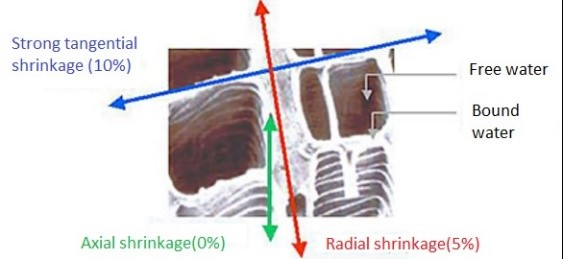
\includegraphics[width=10cm]{fig6}
	\caption{3 types of wood shrinkage}
	\label{fig:galaxy}
\end{figure}

\subsection{Influence of density on wood}

Density is the ratio of the density of wood to that of water. Wood can change in weight and volume as a result of moisture gain and loss. Generally, the reference density is calculated with 12\% moisture. In fact, some researchers have shown that Young's modulus, Poisson's ratio and shear modulus depend on wood density. The density of wood varies from one species to another and also within the same species. The more fibers the wood has, the denser it is. If we take the example of balsa, it has a low proportion of fibers and therefore a low density. Conversely, panacoco has a high proportion of fibers and therefore a high density (\cite{Thibaut2015phd}).

\cite{BodigandJayne1982}  developed a formula \ref{eq:eq12} that relates the mechanical properties of the generalized Hooke's law to the density of wood by the relation :

\begin{equation}
	Y = a*D^b
	\label{eq:eq12}
\end{equation}

where Y represents the elastic properties, D is the density of the wood, a and b are two constants given in the charts for each wood species.

The density is expressed by the formula \ref{eq:eq13}:

\begin{equation}
	D = \frac{\rho_{woodspecimen}}{\rho_{4degreewater}}
	\label{eq:eq13}
\end{equation}

\subsection{Mechanical properties}

From a mechanical point of view, wood is an anisotropic material (= physical and mechanical properties depending on the direction considered) and orthotropic (it has 3 preferred directions: axial, radial, tangential). 

Wood is considered as an elastic material. It means that wood will return to its original shape or dimensions when the load causing the deformation is removed. Beyond this load limit, the wood does not regain its shape. It has then reached the plastic domain. It is the presence of cellulose that gives the wood a linear elastic behaviour. By drawing the stress-strain curve, it is possible to determine the Young's modulus E.


\begin{figure}[htp]
	\centering
	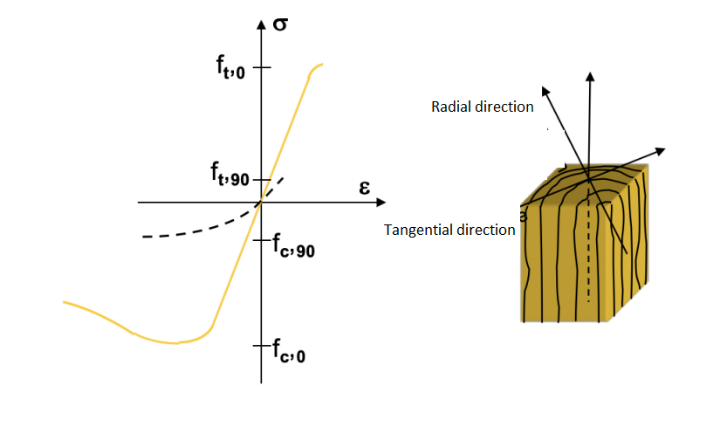
\includegraphics[width=10cm]{fig7}
	\caption{Orthotropy of wood without defects \cite{Taazount2021}}
	\label{fig:fig7}
\end{figure}

The curves in Figure \ref{fig:fig7} show the compressive and tensile behaviour of flawless wood loaded parallel to the fibres (solid line) and perpendicularly (dashed line) at a constant strain rate. Cellulose provides high mechanical properties in the longitudinal direction, as this is the direction in which it is oriented. In the transverse direction, the little cohesion provided by the lignin is not sufficient to hold the fibres together, only the radial tracheids provide a little strength. It can be said that wood without defects has a strong anisotropy. It is rigid and strong parallel to the fibres, sensitive to splitting and has low shear strength \cite{Taazount2021}.

Considering a one-dimensional behavior model in the direction of the fibers, we can write \ref{eq:eq14} :

\begin{equation}
	\sigma = E_{L}*\epsilon
	\label{eq:eq14}
\end{equation}

With the proportionality between the stress $\sigma$ and the deformation $\epsilon$ along the fiber axis with respect to the wood grain, $ E_L $ represents the "longitudinal modulus of elasticity" which must in all rigor be characterized for each load case in tension, compression, bending etc.


\textbf{Compressive behaviour}

In order to determine the behaviour of the material in compression, it must be stressed in both directions (parallel and orthogonal to the fibres). This is known as axial compression and transverse compression. The test is carried out on a parallelepipedic specimen, 20 x 20 x 60  with a loading speed of 40 MPa/mm. The variation of the stress as a function of the strain is plotted in the figure \ref{fig:fig8}.


\begin{figure}[htp]
	\centering
	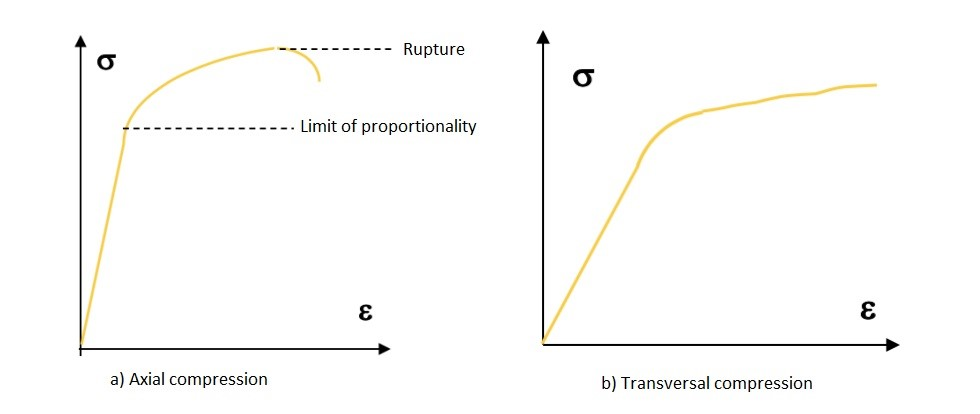
\includegraphics[width=10cm]{fig8}
	\caption{Axial and transverse compression of wood}
	\label{fig:fig8}
\end{figure}

Orders of magnitude of axial compressive strengths and elastic moduli can be given for each type of wood species in table \ref{fig:fig9}. 

\begin{table} \centering
	\begin{tabular}{ccc}
		\toprule % horizontal line at the top of the table
		& Resinous wood & Deciduous wood  \\\midrule
		Axial compression strength & 45 \unit{\mega\pascal}
		& 55 \unit{\mega\pascal} \\\midrule
		Elasticity modulus & 12000 \unit{\mega\pascal}
		& 14000 \unit{\mega\pascal} \\
		\bottomrule % horizontal line at the bottom of the table
	\end{tabular}
	\caption{Orders of magnitude of axial compressive strengths and elastic moduli}
	\label{fig:fig9}
\end{table}


For transverse compression and regardless of the wood species, the strength is divided by 7 (i.e. strength < 10 MPa). 

The strength of the wood can then be assessed if it is loaded obliquely, i.e. the direction of loading is at an angle of 0 to 90° to the direction of the fibres. 


\begin{figure}[htp]
	\centering
	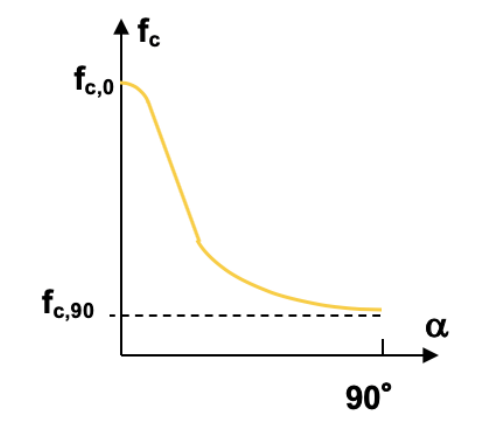
\includegraphics[width=8cm]{fig10}
	\caption{Variation of the compressive strength of wood as a function of the load angle}
	\label{fig:fig10}
\end{figure}

Figure \ref{fig:fig10} shows the variation of the compressive strength of wood as a function of the load angle. It can be seen that the strength is maximum for a load parallel to the fibres (fc,0) and minimum for a load perpendicular to the fibres (fc,90). Theoretically, the compressive strength can be evaluated as a function of this angle using the Hankinson formula. A similar formula \ref{eq:eq15} exists for the modulus.

\begin{equation}
	\sigma_{\alpha} = \frac{\sigma_{0}*\sigma_{90}}{\sigma_{\alpha}*sin(\alpha)^2+\sigma_{90}*cos(\alpha)^2}
	\label{eq:eq15}
\end{equation}

\textbf{Tensile behaviour}

Wood has an almost elastic tensile behaviour until it breaks. Its tensile elastic modulus is equivalent to that in axial compression. The breaking stress is up to twice as high as that in compression. We can retain $f_{t0}=80$ to 140 MPa.


\begin{figure}[htp]
	\centering
	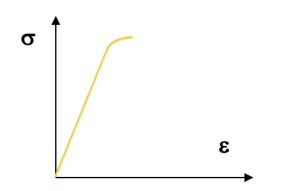
\includegraphics[width=8cm]{fig11}
	\caption{Variation of the axial tensile stress of wood with deformation}
	\label{fig:galaxy}
\end{figure}

In the same way as for compression, the oblique tensile strength can be theoretically evaluated using the Hankinson formula. However, these values are strongly influenced by the presence of knots and the possible slope of the wood grain.

\smallskip

\textbf{Shearing behaviour}

In order to measure the shear strength of wood in the longitudinal direction, a preferential shear plane must be created by the shape of the specimen. This is illustrated in Figure \ref{fig:fig12} :


\begin{figure}[htp]
	\centering
	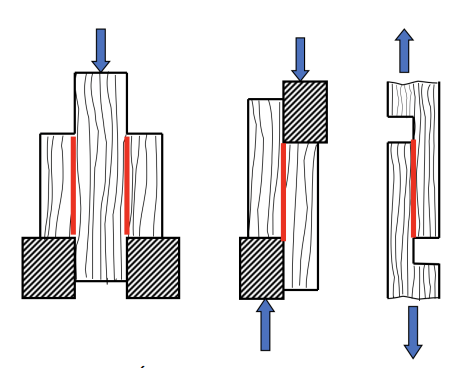
\includegraphics[width=8cm]{fig12}
	\caption{Wood shearing}
	\label{fig:fig12}
\end{figure}

In the figure, the light areas represent the wood, the dark areas represent the blocking points (prevented displacement) and the arrows represent the stresses. These experimental set-ups allow the creation of shear planes (in red). These shear strength values can be retained in table \ref{fig:fig13}.

\begin{table} [H]
\centering
\begin{tabular}{cccc}
	\toprule % horizontal line at the top of the table
	& Resinous wood & Soft deciduous wood & Hard deciduous wood \\\midrule
Shear strenght & 2.5 -- 3.5 \unit{\mega\pascal}
	& 3 -- 5 \unit{\mega\pascal} & 5 -- 7.5 \unit{\mega\pascal}\\
	  \bottomrule % horizontal line at the bottom of the table
\end{tabular}
	\caption{Shear strenght values}
	\label{fig:fig13}
\end{table}

%
%\begin{table}[htp]
%	\centering
%	
\includegraphics[width=10cm]{fig13}
%	\caption{Shear strenght values}
%	\{fig:fig13}
%\end{table}


\section{Fracture mechanic of wood}

\subsection{Test pieces used in fracture mechanics}

There are three ways of applying a force to allow a crack to propagate as shown in figure \ref{fig:fig14}. Mode I is a tensile stress normal to the crack plane, mode II is a shear stress acting parallel to the crack plane and perpendicular to the crack front. Mode III is a shear stress acting parallel to the crack plane and parallel to the crack front. In general, a crack propagates in a material under a combination of stresses in all three modes. These modes can be presenting by the energy release rate (G) linked to crack length. It is called R-curve and has three characterized propagation crack zones. A first increasing phase of instability to initiate the cracking process. A second phase, which corresponds to a stabilised propagation range during which only viscoelastic effects (creep) will participate in the advance of the crack front and a last phase which symbolises the ruin of the material.


\begin{figure}[htp]
	\centering
	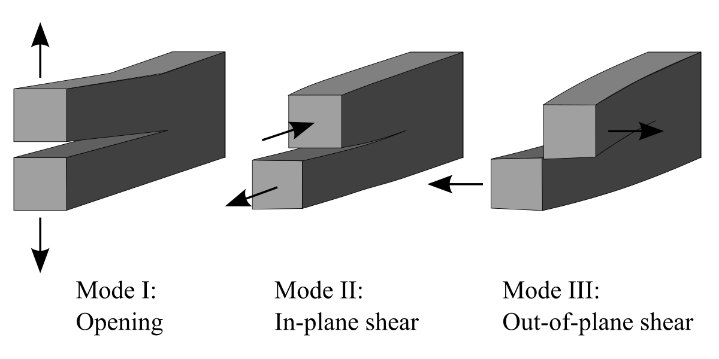
\includegraphics[width=10cm]{fig14}
	\caption{Illustration of the three modes of rupture}
	\label{fig:fig14}
\end{figure}

Moreover, the cracking failure mechanism can occur in two types of cracking: 

\begin{itemize}
	\item Abrupt cracking: for solids, or for very high strength materials, the working stresses are very high, and considerable potential energy is thus created; the presence of small cracks can then lead to abrupt failure which is often not accompanied by macroscopic plastic deformations due to the very low ductility. 
	\item Successive cracking: this is a succession of mechanisms (brittle - ductile) which, under repeated stresses, leads to successive cracking or fatigue failure. The factors that influence the cracking behaviour of materials are of two kinds: metallurgical and mechanical. The mechanical factors relate to the state of displacements, strains and stresses, as well as environmental conditions such as temperature or relative humidity. It is easier to observe because it takes more time to involve samples destruction than a unique and sudden crack. With a material like wood, successive cracks rupture are expected.
\end{itemize}

In order to realize these different modes of rupture, we need specimens that meet certain criteria such as geometry. Indeed, some specimens were designed to solve problems for mode I while others for mode II or mixed mode. There are therefore several types of test specimens:

\textbf{DCB test piece}

The double cantilever beam (DCB) specimen was developed for testing in the crack opening mode (Mode I). Its design allows to obtain a stress intensity factor that decreases when the crack propagates. However, it also allows the determination of the toughness and the critical energy restitution rate in mode I and mode II. Indeed, in the document of \cite{YoshiharaandNobusue2008} Mode I and Mode II fracture toughness were measured of compressed spruce by a double cantilever beam (DCB) test and a three-point bend end notched flexure (3ENF) test figure \ref{fig:fig15}.


\begin{figure}[htp]
	\centering
	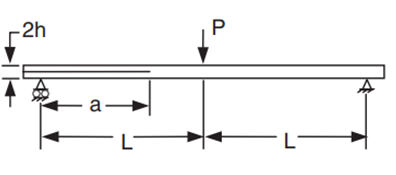
\includegraphics[width=.6\textwidth]{fig15}
	\caption{Schematic representation of 3ENF test with DCB test piece. \cite{DavidsonandSun2005}}
	\label{fig:fig15}
\end{figure}

\newpage
\textbf{Double Cantilever Beam specimen with variable inertia}

The classical DCB specimen had an instability from the beginning of the crack initiation. This is why \cite{Dubois2002} proposed a variable inertia DCB specimen with crack stability. The DCB specimen with variable inertia figure \ref{fig:fig16} was designed to ensure stabilised propagation in Mode I. Thus, after the crack initiation zone, a decrease in the rate of elastic energy restitution G is observed over a given propagation range. During this phase, only viscoelastic effects will participate in the progression of the crack front when the specimen is loaded in creep. The viscoelastic characteristics will thus be clearly decoupled from the cracking parameters. 


\begin{figure}[htp]
	\centering
	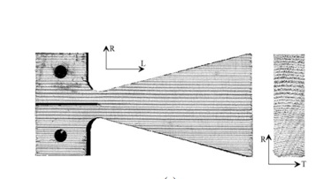
\includegraphics[width=.6\textwidth]{fig16}
	\caption{DCB specimen with variable inertia \cite{Dubois2002}}
	\label{fig:fig16}
\end{figure}


\textbf{Compact Tension Shear specimen}

The Compact Tension Shear (CTS) specimen figure \ref{fig:fig17} is designed to evaluate all mixed modes in different materials. It was developed for mixed loads in isotropic materials. Two steel arms are pierced with holes where symmetrical forces P oriented by angles $\beta$ of mixtures are applied. On both specimens, the crack remains oriented in the direction of high orthotropy.

\begin{figure}[tp]
	\centering
	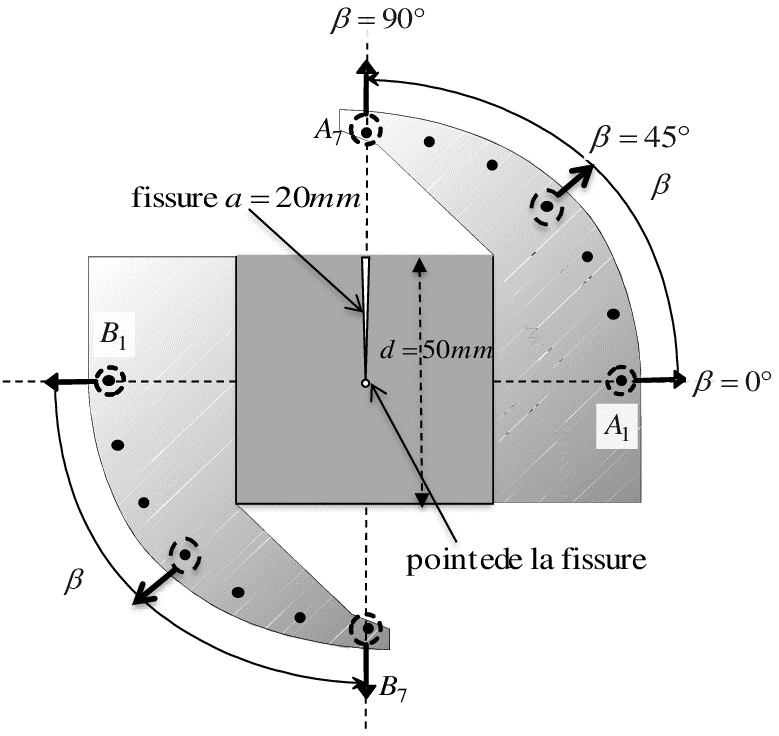
\includegraphics[width=.4\textwidth]{fig17}
	\caption{Compact Tension Shear (CTS) specimen}
	\label{fig:fig17}
\end{figure}

\textbf{Mixed Mode Crack Growth specimen}

The design of the Mixed Mode Crack Growth (MMCG) specimen figure \ref{fig:fig18} was based on a combination of the two geometric solutions described above. The original DCB specimen was modified by adding a lower heel to secure the mixed mode loading device. The upper heel was slightly inclined to ensure stiffness in the vicinity of the two connection fillets. The body of the specimen has increasing inertia towards the crack tip to ensure a stable rate of energy restitution. Four symmetrically arranged PVC arms are attached to the wooden specimen. Boreholes are provided to allow for loads with a variable $\beta$-mixing rate identical to that of the CTS specimen. This test piece allows for a given propagation range, in mode 1, mode 2 and in mixed mode, a stability or even a considerable decrease of the energy restitution rate\cite{MoutouPitti2008}.





\begin{figure}[tp]
	\centering
	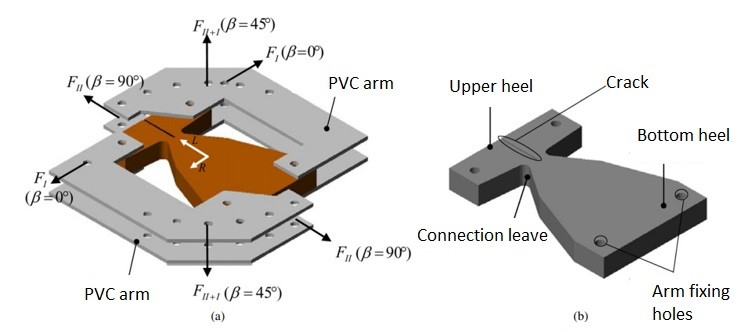
\includegraphics[width=.6\textwidth]{fig18}
	\caption{2MCG test piece \cite{MoutouPitti2008}}
	\label{fig:fig18}
\end{figure}

\subsection{Stress and strain fields}

It is important to notice that different zones are studied. In fracture mechanics, three successive zones visible in figure \ref{fig:fig19} can be distinguished schematically in a cracked medium:

\begin{itemize}
	\item The development zone or zone 1: the zone closest to the crack tip. In this part the material is very damaged, which makes its mechanical evaluation rather complex. The size of this zone determines the type of cracking that will occur. Indeed, if the size of the zone is large, ductile cracking will be observed. On the other hand, if it is small, brittle cracking will be observed.
	\item The singular zone or zone 2: this covers the entire development zone. In this zone, the displacement, strain and stress fields are continuous and have a formulation that is independent of the distant geometry of the structure. The material has a linear viscoelastic behaviour. Its boundary with zone 1 is assumed to be continuous in stress and displacement.
	\item The far zone or zone 3: this is the zone furthest from the crack. It connects the singular zone with the loading and displacement boundary conditions.
\end{itemize}


\begin{figure}[htp]
	\centering
	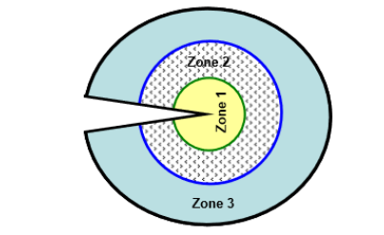
\includegraphics[width=10cm]{fig19}
	\caption{Cracking zone \cite{MoutouPitti2008phd}}
	\label{fig:fig19}
\end{figure}

For a linear elastic material, the stress field at a point M in the vicinity of the crack can be expressed simply as a function of the stress intensity factor $K_{I,II,III}$ and the polar coordinates ( r, $\theta$). The dimensionless functions $f_{ij}$  and  $g_{ij}$ depend on the mode of loading. The intensity factor is independent of point M. Moreover, in the vicinity of the crack tip the value of r is very small, and tends to 0. Thus, the stress field is expressed by \ref{eq:eq16}:

\begin{equation}
	\sigma_{i,j} = \frac{K_{\beta}}{\sqrt{2*\pi*r}}*f_{i,j}(\theta)
	\label{eq:eq16}
\end{equation}

The coefficient $K_\beta$ in the equation \ref{eq:eq16} is the stress intensity factor (mode I and mode II) and is independent of the point M, Figure \ref{fig:fig20}.


\begin{figure}[htp]
	\centering
	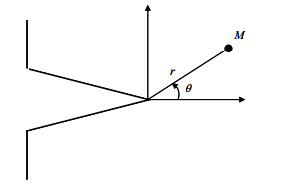
\includegraphics[width=8cm]{fig20}
	\caption{Crack tip scoring}
	\label{fig:fig20}
\end{figure}

We have seen that there are three ways of applying a force, to a specimen, to allow a crack to propagate. These modes define the expression of the mechanical field in zone 2 for orthotropic material \cite{Odounga2018phd}. They are defined and expressed as follows and are illustrated in Figure \ref{fig:fig14}:

\textbf{Mechanical fields in the singular zone for mode 1}

\begin{equation}
	\sigma_{1,1} = \frac{K_{1}}{\sqrt{2 \pi r}} \cos{\frac{\theta}{2}}  \left( 1-\sin{\frac{\theta}{2}} \sin{\frac{3 \theta}{2}} \right)
	\label{eq:eq17}
\end{equation}

\begin{equation}
	\sigma_{2,2} = \frac{K_{1}}{\sqrt{2 \pi*r}} \cos{\frac{\theta}{2}}  \left( 1+\sin{\frac{\theta}{2}} \sin{\frac{3 \theta}{2}} \right)
	\label{eq:eq18}
\end{equation}

\begin{equation}
	\sigma_{1,2} = \frac{K_{1}}{\sqrt{2 \pi r}} \cos{\frac{\theta}{2}}  \sin{\frac{\theta}{2}} \cos{\frac{3 \theta}{2}}
	\label{eq:eq19}
\end{equation}

The displacement field for the mode 1 loading is written as follows:

\begin{equation}
	u_{1} = \frac{K_{1}}{4 \pi}*\sqrt{\frac{r}{2 \pi}} \left((2 \chi-1) \sin{\frac{\theta}{2}}-\sin{\frac{3 \theta}{2}}\right)
	\label{eq:eq110}
\end{equation}

\begin{equation}
	u_{2} = \frac{K_{1}}{4 \pi} \sqrt{\frac{r}{2*\pi}} \left((2 \chi+1) \sin{\frac{\theta}{2}}-\sin{\frac{3 \theta}{2}}\right)
	\label{eq:eq111}
\end{equation}

With : 

$K_1$  the mode 1 stress intensity factor

$\mu=\frac{E}{2 (1+\nu)}$ , the shear coefficient of Lame

$\nu=\frac{\lambda}{2 (\lambda+\mu)}$ , the shear coefficient of Poisson

$E=\frac{\mu (3 \lambda+2 \mu)}{\lambda+\mu}$, the Young modulus

$\lambda=\frac{\nu E}{(1-2 \nu)(1+\nu)}$ , the Lame’s Coefficients

The term $\chi$ is a constant defined as follows:\ $\chi=3-4\nu$ for plane deformations and \ $\chi=\frac{3-\nu}{1-\nu}$  for plane stresses.

r and $\theta$ polar coordinates of point M centred on the crack tip, Figure 11

\smallskip

\textbf{Mechanical fields in the singular zone for mode 2}

\begin{equation}
	\sigma_{1,1} = \frac{-K_{2}}{\sqrt{2 \pi r}} \sin{\frac{\theta}{2}}  \left( 2+\cos{\frac{\theta}{2}} \cos{\frac{3 \theta}{2}} \right)
	\label{eq:eq112}
\end{equation}

\begin{equation}
	\sigma_{2,2} = \frac{K_{2}}{\sqrt{2 \pi r}} \cos{\frac{\theta}{2}}  \sin{\frac{\theta}{2}} \cos{\frac{3 \theta}{2}}
	\label{eq:eq113}
\end{equation}

\begin{equation}
	\sigma_{1,2} = \frac{K_{2}}{\sqrt{2 \pi r}} \cos{\frac{\theta}{2}}  \left( 1-\sin{\frac{\theta}{2}} \sin{\frac{3 \theta}{2}} \right)
	\label{eq:eq114}
\end{equation}

The displacement field for the mode 2 loading is written as follows:

\begin{equation}
	u_{1} = \frac{-K_{2}}{4 \pi} \sqrt{\frac{r}{2 \pi}} \left((2 \chi+3) \sin{\frac{\theta}{2}}+\sin{\frac{3 \theta}{2}}\right)
	\label{eq:eq115}
\end{equation}

\begin{equation}
	u_{2} = \frac{K_{2}}{4 \pi} \sqrt{\frac{r}{2 \pi}} \left((2 \chi+3) \cos{\frac{\theta}{2}}+\cos{\frac{3 \theta}{2}}\right)
	\label{eq:eq117}
\end{equation}

With : $K_2$  the mode 2 stress intensity factor

\smallskip

\textbf{Mechanical fields in the singular zone for mode 3}

\begin{equation}
	\sigma_{1,3} = \frac{-K_{3}}{\sqrt{2 \pi r}} \sin{\frac{\theta}{2}}
	\label{eq:eq118}
\end{equation}

\begin{equation}
	\sigma_{2,3} = \frac{K_{3}}{\sqrt{2 \pi r}} \cos{\frac{\theta}{2}}
	\label{eq:eq119}
\end{equation}

The displacement field for the mode 3 loading is written as follows:

\begin{equation}
	u_{3} = \frac{-2 K_{3}}{\mu} \sqrt{\frac{r}{2 \pi}} \sin{\frac{\theta}{2}}
	\label{eq:eq120}
\end{equation}

With : $K_3$  the mode 3 stress intensity factor

\subsection{Method of the complacency}

In this part we give and define the different terms of the imposed displacement complacency formula. This formula will be used in the next chapters to calculate the energy restitution rate. It is defined by the ratio of two parameters: the variation of energy per unit area cracked and the crack propagation in a linear elastic material. The crack propagation will occur when the energy G reaches a critical value noted Gc. This value Gc is a measure of the toughness of the material. In concrete terms, G defines an overall energy parameter that accounts for the change in potential energy that accompanies the propagation of a crack in a structure. Let us now define the mathematical expression of G. First, let us consider a material with a crack of length a and thickness b. A crack propagation $\Delta$a will be accompanied by the following energy variations \ref{eq:eq121}:

\begin{equation}
	\Delta W_{ext}=\Delta W_{elast}+\Delta U
	\label{eq:eq121}
\end{equation}

With:

$\Delta W_{ext}$ the applied energy change (due to external forces)

$\Delta W_{elast}$ the change in dissipated energy 

$\Delta$U the energy expended during crack propagation over the length $\Delta$a.

The energy G reported to the unit area will be \ref{eq:eq122} :

\begin{equation}
	G = \lim_{\Delta \to 0}= \frac{\Delta U}{\Delta A}= \frac{\partial U}{\partial A}
	\label{eq:eq122}
\end{equation}

Where $\Delta A=b\Delta a$  is the cracked area during crack propagation. b is usually equal to 1 because a unit thickness is often considered. Therefore, the energy per unit thickness will be of the form \ref{eq:eq123} :

\begin{equation}
	G = \lim_{\Delta \to 0}= \frac{\Delta U}{\Delta a}= \frac{\partial U}{\partial a}
	\label{eq:eq123}
\end{equation}

In order to understand the meaning of the energy restitution rate, we will consider, from an initial configuration, the propagation (in a specimen of unit thickness) in the following two classical cases (Figure 18):

\begin{itemize}
	\item propagation with imposed displacement d ; 
	\item propagation with imposed force F.
\end{itemize}

\begin{figure}[htp]
	\centering
	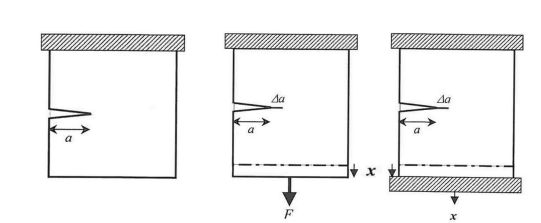
\includegraphics[width=10cm]{fig21}
	\caption{Stable propagation with imposed force or imposed displacement \cite{Zeghloul2001phd}.}
	\label{fig:fig21}
\end{figure}

In our work we will limit ourselves to the case of propagation with imposed displacement. In this case if $\Delta x=0$ (with $\Delta x$ variation of the crack), the external energy variation will be zero, we then deduce the elastic energy :

$W_{elast}=\frac{Fx}{2}$

By introducing the complacency by the relation :

$C=\frac{x}{F}$

We deduce :

$W_{elast}=\frac{CF^2}{2}=\frac{x^2}{2C}$

$\Delta W_{elast}=\frac{\partial W_{elast}}{\partial a}\Delta a=\frac{\partial W_{elast}}{\partial a}\ \frac{\partial C}{\partial a}\Delta a=\frac{-x^2}{2C^2}\ \frac{\partial C}{\partial a}\Delta a$

And because we have:

$\Delta W_{ext}=0=\Delta W_{elast}+\Delta U\leftrightarrow \Delta U =-\Delta W_{elast}$

Then we have:

$\Delta U=\frac{x^2}{2C^2}\ \frac{\partial C}{\partial a}\Delta a$

Which enables to obtain \ref{eq:eq124}:

\begin{equation}
	G=\frac{x^2}{2C^2}\ \frac{\partial C}{\partial a}=\frac{F^2}{2}\ \frac{\partial C}{\partial a}
	\label{eq:eq124}
\end{equation}

The relationship in equation \ref{eq:eq124} is related to the unit thickness. In the case where $b\neq1$
we obtain \ref{eq:eq125}:

\begin{equation}
	G_c=\frac{{F_{ci}}^2}{2b}\ \frac{\partial C}{\partial a}
	\label{eq:eq125}
\end{equation}

With:

$G_c$ the value of energy release rate (in $J/mm^2$)

$F_{ci}$ the critical force which involves the crack (in N)

b the thickness of the specimen (in mm)

C the complacency evolution (in ${Pa}^{-1}$)

a the crack length evolution (in mm)



\section{Software and DIC method}

\subsection{Dic method}

Digital image correlation (DIC) was developed in 1983. It is a 2D or 3D optical method that measures displacements between two images. It is increasingly used in materials science to determine strain fields, detect cracks or provide displacement fields for material property identification procedures. It is a non-contact optical method of measuring kinematic fields, based on the comparison of the signal amplitude. It relies on the grey levels of the images. The particles are optically tracked using computer algorithms to determine displacements and velocities. Rather than tracking moving particles in a fluid, DIC tracks changes in the relative position of the high contrast surface finish. It works by comparing two images, one reference and one deformed, taken during loading. Thus, it must detect a pattern in the reference image and compare it to the pattern in the other images \cite{Mambili2018}. The DIC formulation relies on the conservation of grey levels between the two instants at which the reference images S0 and the current images St are recorded. In other words, this principle is based on the comparison between a reference image and a distorted image. Each image is composed of pixels, and each pixel as a function of the light flux returns information. For 8-bit images, for example, a pixel can have a value between 0 for black and 255 for white. Each image is therefore stored in the form of a two-dimensional matrix whose cells correspond to a value. These matrices are the image correlation data. DIC compares these matrices and deduces the surface displacement field. To do this, during the analysis, the algorithm in place searches for a correlation zone, predefined in the reference image, in that of the image in the deformed state figure \ref{fig:fig22}.


\begin{figure}[htp]
	\centering
	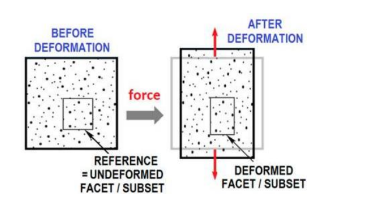
\includegraphics[width=10cm]{fig22}
	\caption{Example of captured images obtained by a camera for image analysis.}
	\label{fig:fig22}
\end{figure}

The system consists of a digital camera and specialised computer software like MatchID. The camera is used to capture consecutive images of the surface of the sample under test before and during the deformation test. The digital images thus determined, which correspond to a series of pictures, are analysed by the DIC software. After the determination of
the displacement field, it is possible to
obtain the strain field.

It is important to note that the 2D orthotropic elastic material model used for wood requires five engineering constants as input parameters in image analysis systems. These inputs are specific to the software used and include the Young's modulus in the longitudinal direction ($E_L=E_1$), the transverse Young's modulus ($E_{trans}=E_R=E_T=E_2$), and the shear modulus ($G_{LR}=G_{LT}=G_{12}$) if the shear mode is being studied.
The Poisson's ratio $\nu$ is also a necessary input and may vary depending on whether the surface being studied is in or out of the plane. Additionally, the initial crack length must be input into the model.
Three main inputs are required to describe damage, although this may vary depending on the software being used. For mode I damage, the damage initiation stress ($\sigma_{ini}$), the failure stress ($\delta_{fl}$), and the shape coefficient of the exponential function ($\alpha_l$) are used to describe the damage.

\subsection{Uncertainty Quantification}

There are two types of errors in DIC measurements, namely variance errors and bias errors. The main sources of noise in DIC measurements are camera noise and matching errors during the correlation process. Bias can be introduced by smoothing of spatial gradients in a QOI, uncorrected lens distortions, poor camera calibration, and out-of-plane motion in 2D-DIC measurements, to name a few sources. Establishing the uncertainty of the QOIs accounting for bias and noise errors is essential for intelligent evaluation and use of DIC results. Without quantifying the uncertainty, it is impossible to know whether a reported QOI value is meaningful and relevant, or whether it is the result of random noise and bias.

Bias errors are often difficult to quantify, as the true value of a QOI is usually not known. However, some sources of bias can be assessed. Even if no bias errors are detected, unknown bias errors may still exist.

The process of quantifying variance errors is often called noise floor analysis. The basic idea of a noise floor analysis is to correlate static images of a DIC pattern that were acquired under the same conditions as the test images. With no force applied or displacement on the test piece, all measured QOIs requiring deformation are errors. The same user-selected DIC parameters that are used for the analysis of the test piece images during deformation should also be used for the analysis of the noise floor images. Therefore, the final noise floor analysis is typically performed after the mechanical test image analysis, but using the images acquired immediately before the mechanical test.
Two different metrics can be used to quantify the variance error of the QOIs: a spatial standard deviation and a temporal standard deviation. It is recommended that both spatial and temporal standard deviations are calculated and evaluated to see if one is significantly larger than the other. However, the spatial and temporal standard deviations are generally similar, and a single metric or the average of the two metrics can be selected to quantify the noise floor. 

%To quantify the spatial variation of the QOI, compute the standard deviation of the QOI for each image and average this spatial standard deviation over time for all static images. To quantify temporal variation, calculate the standard deviation of the QOI for each subset over time and average this temporal standard deviation for each subset over all subsets in the image ZOI.

\section{Conclusion}

This chapter has provided a better understanding of the material wood. Its definition, its various functions, its physical and mechanical properties were reminded, as well as the elements that constitute it at the macroscopic and microscopic levels. Moreover, it was also recalled that various parameters such as moisture can influence the physical and mechanical characteristics of wood.
This chapter also recalled some basics of fracture mechanics and different specimens used for the observation of crack propagation. In particular, it explains the choice of using the 2MCG specimen for the tests. It also recalls the basic formulas of linear fracture mechanics in an orthotropic field, such as the stress intensity factors and the energy restitution rate. In addition, the field measurement method called DIC was presented and the procedure to obtain the crack propagation was explained. The next chapter will present the applied experimental method.


